\section{Background}
%Next we give an overview on background information and the attacking scenario essential for understanding the key principles that underlie our proposed protection methods.

\subsection{Android Dex Bytecode}
Typically, Android applications are programmed using Java. The application source code is compiled to the Dex bytecode format which is then packed into a Android application package (APK) together with application resources (such as images and configuration files). 
The Dex bytecodes can be either dynamically interpreted (using the Dalvik VM before Android 5.0) or compiled into native machine code during installation by the Android Runtime since Android 5.0. Our approach only applies to the Dex bytecode without changing the Android VM or compilation process. Hence, our approach is portable across different Android versions. 





%and deployed as files with an ".apk" suffix, later called APK. It is basically a ZIP-compressed file and contains resources of the application like pictures and layouts as well as a dex file. This dex file, saved as "classes.dex", contains the program code in form of Dalvik bytecode. The content of the APK is also cryptographically signed, which yields no security improvement but helps to distinguish and confirm authenticity of different developers of Android applications. There are two Android virtual machine and the Dalvik VM was replaced by the Android runtime(ART). The difference between them is that ART virtual machine will translate the dex bytecode into native machine code when installing the application, so both virtual machines execute the same unmodified Dalvik bytecode file structure, instruction formats(smali), and constrains. Hence, our proposed obfuscation applies to apps run by both DVM and ART.
%Within the installation process, every installed application gets its own unique user ID by default. This means that every application will be executed as a separate system user. The execution process\cite{08} of an Android application is shown in Figure ~\ref{fig:Figure 3}.

\begin{figure}[!tbp]
  \centering
  % Requires \usepackage{graphicx}
  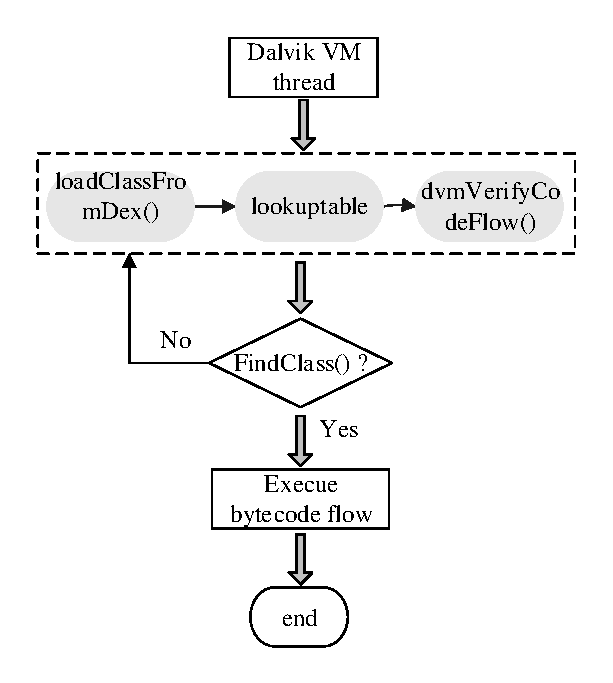
\includegraphics[width=0.8\columnwidth]{fig/fig3.pdf}
  \caption{The process of Dalvik VM execution. this figure presents the Dalvik VM how to execute an Android app\emph{(load, link, verify,run)}.}
  \FIXME{This diagram should go. Dalvik is dead. }
  \label{fig:Figure 3}
\end{figure}


\FIXME{We shouldn't talk of dynamic execution of Dex bytecodes. Again, this is because Dalvik is already dead!}

%In detail, the specific process is as follows:
%\begin{itemize}
%  \item \textbf{Load the Classes.} Firstly, Dalvik VM loads the class by function loadClassFromDex(), and when the classes have been successfully resolved, each class will have a ClassObject type of data structure in the runtime environment. Dalvik VM stores and searches all loaded classes by using gDvm.loadedClassed global hash table;
%  \item \textbf{Verify Bytecode.} Bytecode verifier verifies the loaded class by using function dvmVerifyCodeFlow();
%  \item \textbf{Find the main class.} Dalvik VM searches and loads main method class in gDvm.loadedClassed global hash table by using function FindClass( ). If it can't find the needed class, it will go back to load the class;
%  \item \textbf{Execute bytecode flow.} Initialize the interpreter by invoking function dvmInterpret( ) and execute the bytecode flow.
%\end{itemize}

 The Dex bytecode follows a stack machine where
operands of all operations are stored in a virtual 32-bit register. The only
exception is floating point operands which are always stored using a 64-bit
register. The other key structure of Dex is that function calls always follow by
an instruction to retrieve the return value
of the function. This is a key point where an attacker will focus on when attempting to trace the program control flow using dynamic code analysis.
The binary form Dex bytecode can be dissembled into Smali, a
human readable format of Dex.
To perform code protection, our approach first dissembles the Dex bytecode into Smali;
it then applies code obfuscation on Smali and assemble the obfuscated Smali code back into Dex bytecodes. 

Figure~\ref{} gives an example of the generated Smali code of a simple java
function. \FIXME{Here gives an example of how a Java function is compiled
into Smali. The example should show that the operands are stored in a 32-bit
register and the function call is always follows by an instruction to
retrieve the return value}.



%
%\textbf{smali code.} We can disassemble the contents of the app and generate folder in disassembling project directory, using the android-apktool, which contain all the disassembled smali\cite{03} files. These files will be generated according to the package hierarchy corresponding directory and all classes generate independent smali files in the corresponding directory of the program\cite{20}.
%
%The smali code is a instruction language of Dalvik VM, which is register-based, and frames are fixed in size upon creation. Each frame consists of a particular number of registers(specified by the method)as well as some adjunct data needed to execute the method. When used for bit values(such as integers and floating point numbers), registers are considered 32 bits wide. Adjacent register pairs are used for 64-bit values, such as double and long numbers. All variables of smali code are stored in registers. For example, in the instruction "const-wide v0, 0x0000000400000003 ", it is a definition of the long number, indicating that it operates on wide(64 bit) data, and "v0,v1" is the destination register.


\subsection{The Attacking Model}
%Reverse engineering is the necessary condition that Android applications are repackaged or tampered by attackers. This process aims at enabling an analyst to understand the concrete relation between implementation and functionlity of the program. In this paper we focus on resisting the decompiling process because this is the fundamental step in reverse engineering due to the fact that most of the other processes are based on the decompiling process.

Figure~\ref {fig:Figure 2} illustrates a representative attacking scenario for Android applications. We use this attacking model to evaluate our approach in this paper. To perform the attack, an adversary first extract the Dex file from application APK. The attacker will then xxx.
\FIXME{I have no idea why the attacker will translate dex bytecode into Java code?}
%In recent years, the attackers usually achieve their malicious behaviors. Firstly, they can successfully decompile .dex into .java, which is java source code.But they will not analyze smali code that is after disassembling, because of enormous and complex grammar than Java source code. Therefore, an attacker locate the critical sections from all over the java source codes quickly, then analyze the main function within the smali file\cite{04} or .so native library based on the previous position.The process is as shown in Figure~\ref{fig:Figure 2}.


\begin{figure}[!tbp]
  \centering
  % Requires \usepackage{graphicx}
  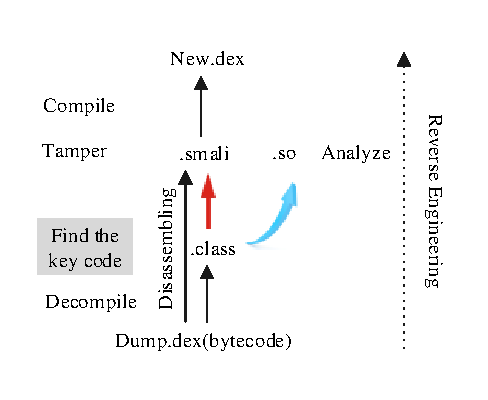
\includegraphics[width=0.8\columnwidth]{fig/fig2.pdf}
  \caption{Reverse engineering. The process that attacker was cracked a app is shown in the figure. }\label{fig:Figure 2}
\end{figure}

We can analyze a instance about online ordering app from Android Open Source Software Community. Firstly, we can see that two variables within java source code is defined in the code of ordering. It is the int-type of the number of clicks and purchase quantity and shown in the following:


\begin{lstlisting}[language={[ANSI]C}, backgroundcolor=\color{backcolour},
numbers=left,numberstyle=\tiny,keywordstyle=\color{blue},commentstyle=\color{red!50!green!50!blue!50}][6pt]
private int CLICK_NUM = 0;
private int buyNum = 0;
\end{lstlisting}

\noindent According to the location, we can quickly find it in the smali code. It is shown in following:

\begin{lstlisting}[language={[ANSI]C}, backgroundcolor=\color{backcolour},
numbers=left,numberstyle=\tiny,keywordstyle=\color{blue},commentstyle=\color{red!50!green!50!blue!50}][6pt]
const/4 v7, 0x0
.local v7, CLICK_NUM:I
const/4 v8, 0x0
.local v8, buyNum:I
\end{lstlisting}

\noindent  If they didn't be protected, the attackers can find their location and then modify their initial value to steal the user's money. In order to resist this kind of attack, we processed a method through obfuscating variables of being stored in registers.

